\documentclass[]{article}

\usepackage[utf8]{inputenc}

\usepackage[T1]{fontenc}

\usepackage[english]{babel}

\usepackage{amsmath, amsfonts, amssymb, amsthm}

\usepackage{fullpage}

\usepackage{enumerate}
\usepackage{graphicx}
\usepackage{algorithm}
\usepackage{algorithmic}

\usepackage{hyperref}
\hypersetup{
    colorlinks,
    citecolor=black,
    filecolor=black,
    linkcolor=black,
    urlcolor=black
}


%Pour les algos
\floatname{algorithm}{Algorithme}
\renewcommand{\algorithmicrequire}{\textbf{Entrée:}}
\renewcommand{\algorithmicensure}{\textbf{Sortie:}}
\renewcommand{\algorithmicif}{\textbf{si}}
\renewcommand{\algorithmicthen}{\textbf{alors}}
\renewcommand{\algorithmicelse}{\textbf{sinon}}

\title{
{\Huge Digital filtering}\\
Signal processing\\
}

\author{
\textbf{Dell’Aria Doriano}\\
\and
\textbf{Goffaux Lionel}
}


\date{\today\\
Academic Year 2020-2021\\
Bachelor's degree in Computer Science\\
\vspace{1cm}
Faculté des Sciences, Université de Mons}

\begin{document}

\maketitle
\pagebreak

\section{Approximation of second order filters}
\subsection*{Band-pass filter:}
\begin{enumerate}
    \item Finding $\theta$ : we computed $\theta = \frac{f}{2\pi}Fe = 1.88$.
    \item Finding $\rho$ : we fixed K = 1 and we drawn this graph representing the height differency between \{120Hz,121Hz\} and \{119Hz,120Hz\}.
    \begin{figure}[h]
        \centering
        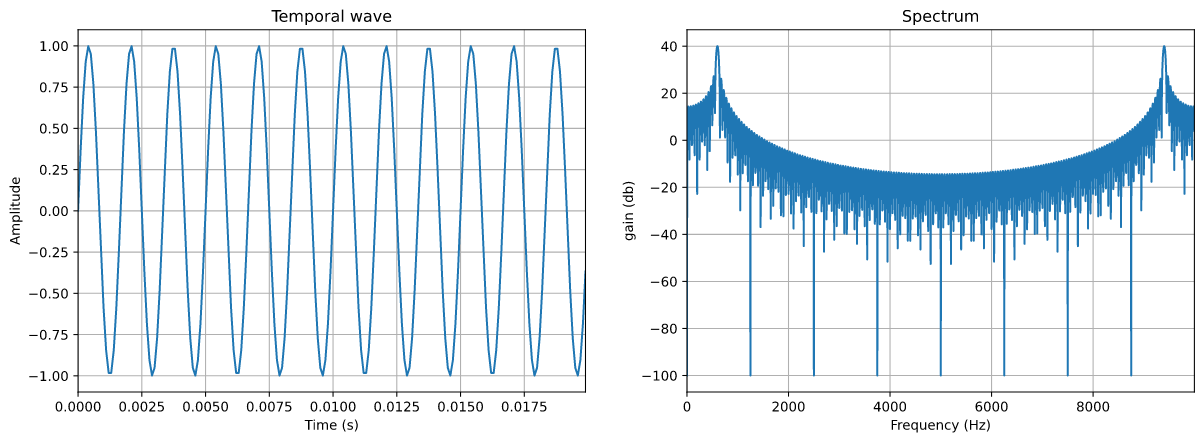
\includegraphics[scale=0.25]{q1.png}
    \end{figure}\\
    we fixed $\rho$ = 0.87
    \item Finding K : we computed $K = \frac{1}{A_{120Hz}}=0.2432$.
\end{enumerate}
The transfer function of the pass-band filter is 
$$H(Z) = K\frac{1 - \cos{(\theta)} Z^{-1}}{1 - 2\rho \cos{(\theta)Z^{-1} +\rho^2Z^{-2}}}$$
where K = 0.2432, $\rho$ = 0.87 and $\theta$ = 1.88.


\subsection*{Stop-band filter:}
\begin{enumerate}
    \item Finding $\theta$ : we computed $\theta = \frac{50}{2\pi}Fe = 0.78$.
    \item Finding $\rho$ : we fixed K = 1 and we drawn this graph representing the attenuation at 49.9 Hz and 50.1 Hz. We want to attenuate these frequency at -47dB
    \begin{figure}[h]
        \centering
        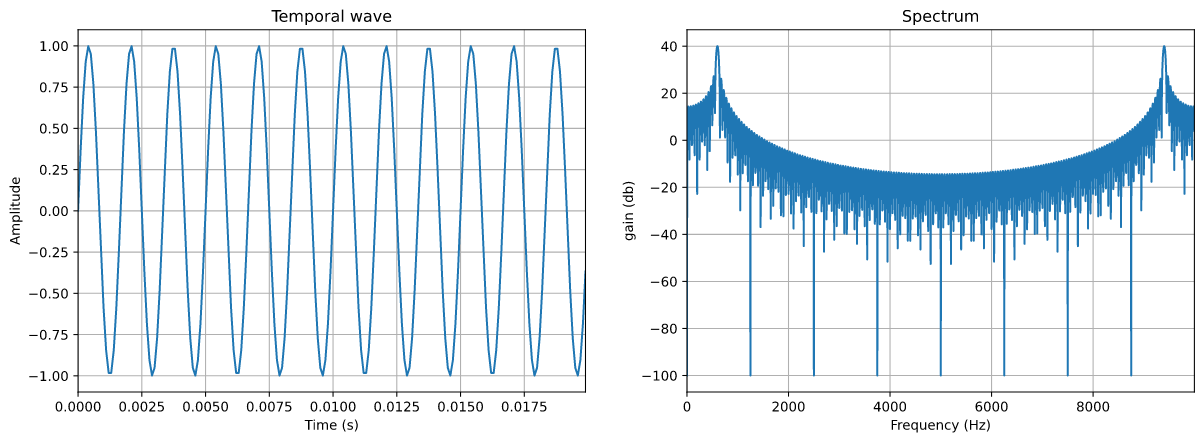
\includegraphics[scale=0.25]{q1.png}
    \end{figure}\\
    we fixed $\rho$ = 0.56
    \item Finding K : we computed $K = \frac{1}{A_{120Hz}}=0.6713$.
\end{enumerate}
The transfer function of the stop-band filter is 
$$H(Z) = K\frac{1 - 2\cos{(\theta)} Z^{-1} + Z^{-2}}{1 - 2\rho \cos{(\theta)Z^{-1} +\rho^2Z^{-2}}}$$
where K = 0.6714, $\rho$ = 0.56 and $\theta$ = 0.78.


\end{document}